\documentclass[11pt,oneside]{article}
\usepackage[margin=1in]{geometry}
%\usepackage{czech}
\usepackage[utf8]{inputenc}
\usepackage[czech]{babel} % nové rozhraní pro použití babelu, ale zatím s ním mám problémy
\usepackage{listings}
\usepackage{graphicx}
\usepackage{python}
\usepackage{mathtools}
%\usepackage{mathtools}
%\usepackage[english]{babel}
\usepackage[hidelinks]{hyperref}
\lstset{language=R}
\DeclareGraphicsExtensions{.pdf,.png,.jpg,.pdf}

\begin{document}
	\title{Aplikace lineární a nelineární filtrace: abstrakce obrazu}
	\author{Jaroslav Hrách\\\\České vysoké učení technické v Praze\\Fakulta informačních technologií}
	\maketitle

\section{Úvod}
\par{V semestrální úloze z předmětu DZO jsem měl za úkol naimplementovat dvě filtrace - lineární a nelineární. Výsledkem těchto filtrů měla být abstrakce obrazu. Aby byl výsledek mé práce více použitelný pro uživatele a nejednalo se jen o demonstraci algoritmů v konzoli či vývojovém prostředí, vytvořil jsem webovou aplikaci s přehledným grafickým rozhraním, které umožňuje nahrát fotografii buď formou formuláře anebo vyfocením přes webovou kameru, podobně jako to mají moderní aplikace jako Instagram.}

\par{Algoritmy pro úpravu obrázků byly implementovány v jazyce Javascript, k webovému rozhraní byl použit front-end framework Bootstrap 3 a manipulace s webovou kamerou pracuje s canvasem z HTML5.}

\section{Teoretický základ}
\par{K docílení abstrakce obrazu se využívá lineární filtrace a nelineární filtrace. Pomocí nelineární filtrace se aplikuje bilaterální filtr a pomocí lineární filtrace detekce hran.}

\subsection{Konvoluce}

Konvoluce je matematicky definovaná následujícím vzorcem:

\[
(F * G)[s, t] = \sum_{x} \sum_{y} F[x][y] \cdot G[s-x][t-y]
\]

kde $F$ představuje zdrojový obrázek a $G$ představuje konvoluční jádro. Operace konvoluce je značena symbolem $*$. Zjednodušeně máme nějaký 2D obrázek po kterém se pohybujeme lineárně konvolučním jádrem, které odpovídá zvolenému rozměru (např. 3x3). Pro každý obrázkový bod se počítá nová hodnota. Ta odpovídá váženému průměru okolních barev, které jsou ještě navíc násobeny odpovídajícím hodnotám v konvolučním jádru. Tento přístup si však nedokáže poradit s ostrými hranamy v obrázku a provádí konvoluci i přes ně. To má za příčinu, že jsou hrany po provedení algoritmu rozmazány. Abychom tomuto problému předešli, musíme použít bilaterální filtr.

\subsection{Bilaterální filtr}

Bilaterální filtr vychází z konvoluce a dbá na zachování ostrých hran u obrázku. Hrana se v tomto případě definuje jako rozdíl jasů sousedících obrazových bodů. Bilaterální filtr je matematicky definován vzorcem:

\[
(F * G_b)[s, t] = \frac{1}{W}\sum_{x} \sum_{y} F[x][y] \cdot G[s-x][t-y] \cdot b(F[x,y] - F[s,t])
\]
\[
W = \sum_{x} \sum_{y} G[s-x][t-y] \cdot b(F[x,y] - F[s,t])
\]

$F$ je opět zdrojový obrázek, $G$ je konvoluční jádro, tentokrát však doplněno o gaussovu funkci $g(y) = a*\exp{-\frac{(x-\mu)^2}{2\sigma^2}}$. Díky ní jsme schopni rozeznat, kde se pravděpodobně nachází ostrá hrana a nedojde tedy aplikací konvoluce k jejímu rozmazání.

Tato značná výhoda bohužel stojí výrazně větší výpočetní čas, neboť se jedná o nelineární operaci. Výpočet hrubou silo odpovídá složitosti $\mathcal{O}(|F|\cdot|G|)$. Bilaterální filtr se dá kromě hrubé síly implementovat i několika dalšími metodami, které se snaží výpočet urychlit - Piecewise-linear, bilateralní mřížka či box kernel.

\subsection{Detekce hran}

Detekce hran se dá implementovat hned několika různými algoritmy. Každý má své výhody a nevýhody. Ve své semestrální práci jsem úspěšně naimplementoval algoritmus využívající Sobelův operátor. Dále jsem se pokusil o detekci hran pomocí Laplaciánu Gaussiánu (LoG).

\subsubsection{Sobel}

Sobelův operátor se používá pro detekci vodorovných a svislých hran, k čemuž se používají právě dvě matice (níže uvedené $G_x$ $G_y$). 

\[
G_x = \begin{bmatrix} 
-1 & 0 & +1  \\
-2 & 0 & +2 \\
-1 & 0 & +1 
\end{bmatrix}
\]

\[
G_y = \begin{bmatrix} 
-1 & -2 & -1  \\
0 & 0 & 0 \\
+1 & +2 & +1 
\end{bmatrix}
\]

Sobel je jednoduchý na implementaci, úspešně odstraní šum a celkem úspěšně detekuje opravdu výrazné hrany. Jeho nevýhodou však je, že když už hrany detekuje, jsou velmi výrazné a tlusté.

\subsubsection{Laplacián Gaussiánu (LoG)}

Další detekce hran využívá lineární Laplaceův operátor (Laplacián) $\nabla^2 f(x,y)$, který vychází z druhých parciálních derivací. Pokud k Laplaciánu přidáme ještě Gaussián $G(x,y) = e^{-\frac{(x-\mu)^2}{2\sigma^2}}$, kde $x$ a $y$ jsou souřadnice pixelu a $\sigma$ je středněkvadratická odchylka, jsme schopni vyhladit původní obrázek a zjemnit hledané hrany. LoG funkce je matematicky definována takto:

\[
LoG(x,y) = -\frac{1}{\pi \sigma^4}[1 - \frac{x^2 + y^2}{2 \sigma^2}]\exp(\frac{x^2 + y^2}{2 \sigma^2})
\]

Detekce hran pomocí LoG má oproti Sobelu výhodu v tom, že výsledné hrany detekuje a zvýrazní mnohem lépe a čistěji. Hrany jsou spíš decentní a při zvýraznění hran lépe dokreslují samotný obrázek. Na druhou stranu je potřeba zvolit správné parametry ($\sigma$ a velikost jádra), aby se hrany detekovaly správně.

\section{Implementace}
\par{Jak jsem zmínil již v úvodu, pro implementaci algoritmů na úpravu obrázků byl zvolen jazyk Javascript, webové rozhraní využívá front-end framework Bootstrap 3 a funkcionalitu webové kamery zajišťuje canvas z HTML5 v kombinaci s Javascriptem.}

\subsection{Konvoluce a bilaterální filtr}

Vzhledem k tomu, že bilaterální filtr vychází z konvoluce, byl naimplementován metodou hrubé síly (tedy se složitostí $\mathcal{O}(|F|\cdot|G|)$), kdy se počítá klasická konvoluce, je násobena gaussovou funkcí, jejíž cílem je rozpoznat ostré hrany a zamezit jejím rozmazáním.

\subsection{Detekce hran}

Pro detekci hran byl nejprve naimplementován relativně přímočarý Sobel detektor, následně byl vyzkoušen i jiný přístup

\subsubsection{Sobel}

Postupoval jsem přesně tak, jak jsem uvedl v teoretickém základu, tedy vytvořil jsem si dvě 3x3 velké matice, kde jedna detekuje vodorovné čáry a druhá detekuje svislé čáry. Ty jsem následně použil při konvoluci.

\subsubsection{Laplacián Gaussiánu (LoG)}

Opět jsem naimplementoval funkci podle matematického předpisu a úspěšně vypočítal matice podle zvolené velikosti a parametru $\sigma$. Bohužel se mi nepodařilo správně doimplementovat detekci nulových hodnot, podle kterých se pozná, že jde o hrany. Nakonec jsem použil aproximovaná jádra o různých velikostech a ty mi při výpočtu dávaly celkem dobré výsledky.

\begin{figure}[!htb]
\centering
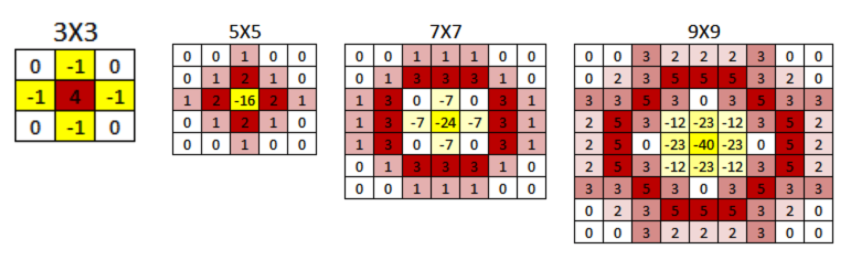
\includegraphics[width=1.0\textwidth]{log-kernel.png}
\caption{LoG - aproximovaná jádra}
\end{figure}

\subsection{Webové rozhraní}

Při práci na semestrální úloze jsem chtěl udělat použitelnou aplikaci, kterou by si mohl vyzkoušet jakýkoliv uživatel. Proto jsem se rozhodl vytvořit jednoduché a přehledné webové rozhraní, ve kterém si uživatel může snadno pořídit svou fotografii, případně nahrát vlastní obrázek a na něm následně pomocí pár kliků aplikovat vybrané filtry.

\begin{figure}[!htb]
\centering
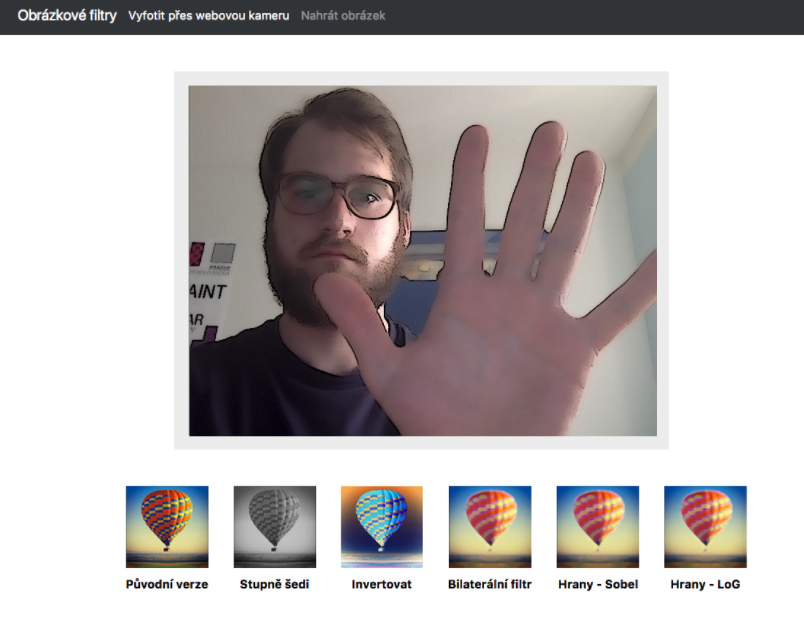
\includegraphics[width=1.0\textwidth]{web-screen-01.png}
\caption{Webové rozhraní aplikace - webová kamera}
\end{figure}

Jelikož jsem filtry programoval v Javascriptu, bylo snadné dodělat webové rozhraní. Pro práci s webovou kamerou je využíván HTML5 tag canvas, který pracuje právě s Javascriptem.

\begin{figure}[!h]
\centering
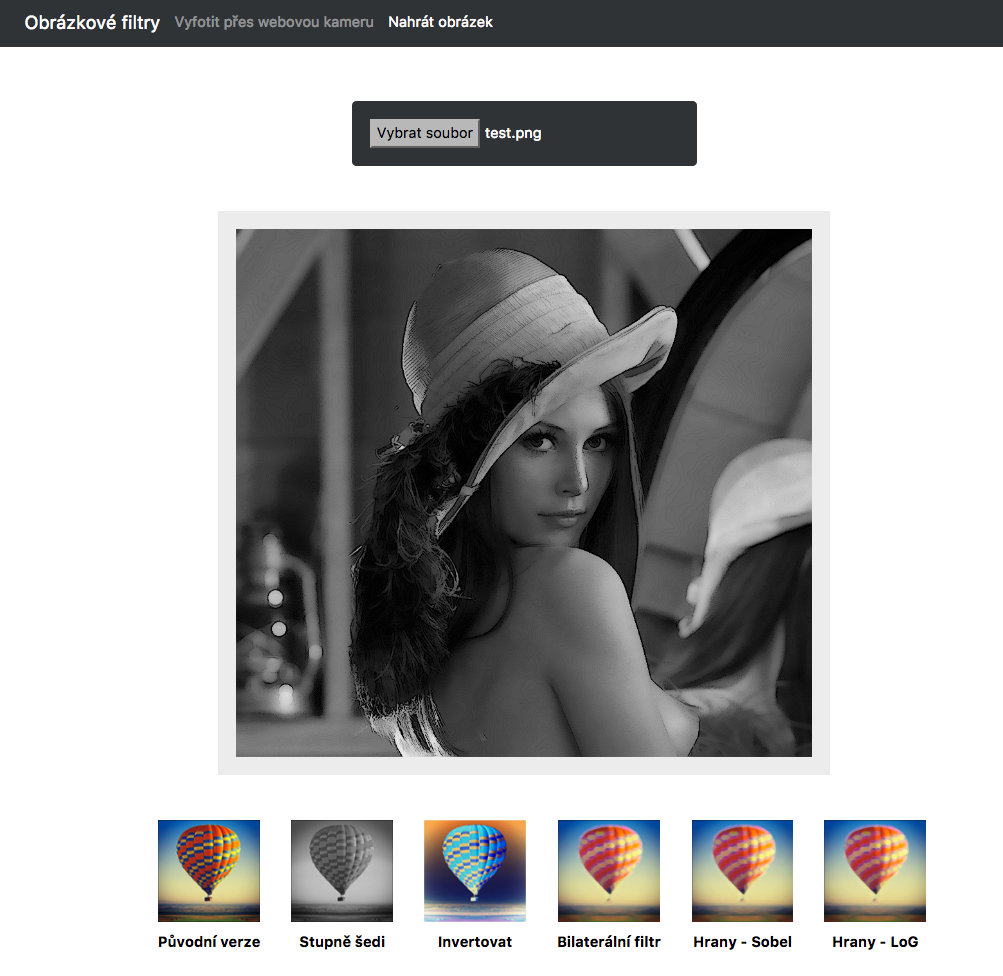
\includegraphics[width=1.0\textwidth]{web-screen-02.png}
\caption{Webové rozhraní aplikace - upload fotky}
\end{figure}

\clearpage

\section{Experimenty}

Při experimentálním vyhodnocení byly nalezeny optimální hodnoty pro proměnné sigma a velikost jádra. Pro testování s jinými hodnotami je potřeba měnit kód v Javascriptu.

\section{Bilaterální filtr}

Efekt bilaterálního filtru se dá zesilovat iterativně a není třeba měnit nastavení parametrů (byly nastaveny hodnoty $\sigma = 4$ a velikost jádra $= 16$). I po třech aplikacích dával filtr relativně použitelný výsledek, obzvlášť, pokud se na něj v samém závěru aplikovalo ještě zvýraznění hran.

\begin{figure}[!htb]
\centering
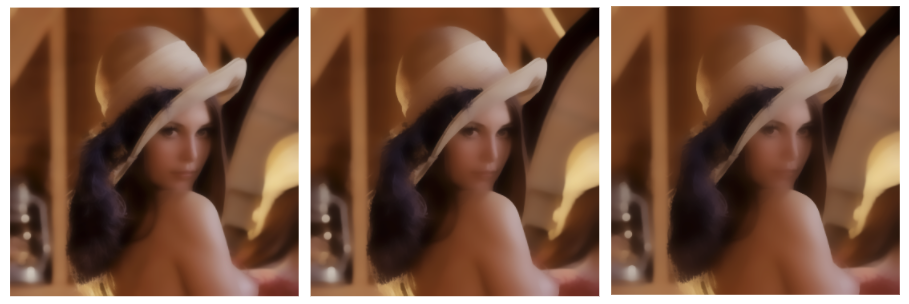
\includegraphics[width=1.0\textwidth]{bilateral-iterative.png}
\caption{Iterativní testování bilaterálního filtru}
\end{figure}

Dále jsem u filtru testoval změny parametrů a pro tři různé velikosti jader (12, 16 a 20) jsem testoval čtyři různé $\sigma$ (4, 5, 6, 10). U malého jádra se efekt rozmazání neaplikoval tak silně, jak bychom chtěli, ale zase byl výpočetně rychlejší (což ale není žádné překvapení, když je bilaterální filtr naimplementován metodou hrubé síly). Intenzita rozmazání se výrazně měnila při změně $\sigma$ a u velkého jádra způsobila už velmi silné rozmazání.

\begin{figure}[!htb]
\centering
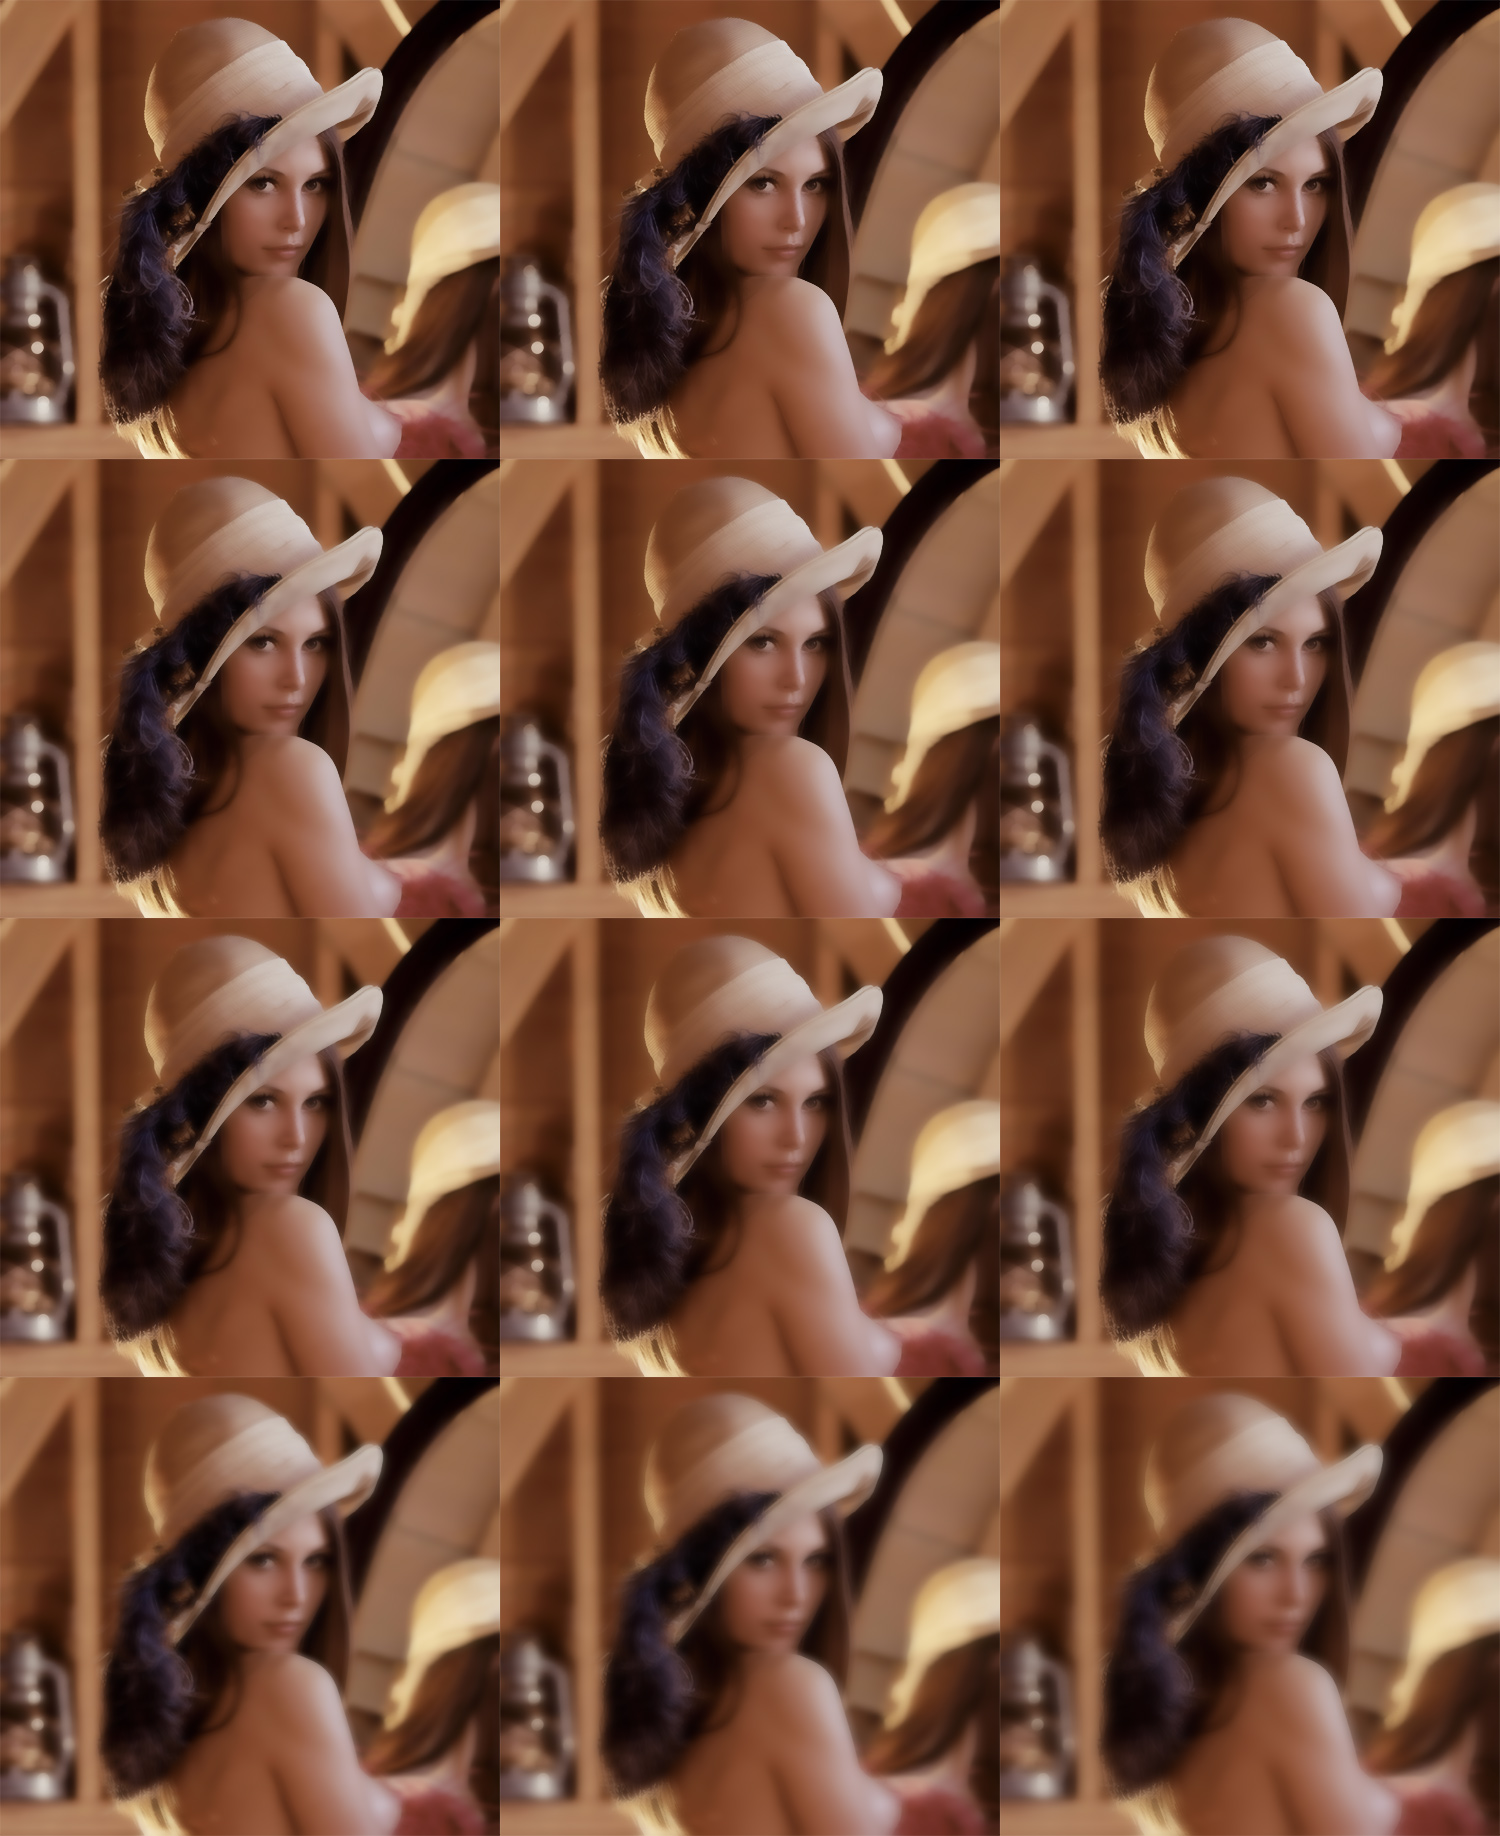
\includegraphics[width=1.0\textwidth]{bilateral-parametry.jpg}
\caption{Změna parametrů u bilaterálního filtru}
\end{figure}

\clearpage

\section{Detektor hran}

Jak jsem popisoval v teoretické sekci, Sobel a LoG dávají poměrně odlišné výsledky. Sobel se zbaví šumu, nicméně dělá celkem viditelné a někdy až nepěkné hrany. Naopak LoG v závislosti na zvoleném jádru dělá pěkné uhlazené hrany.

\begin{figure}[!htb]
\centering
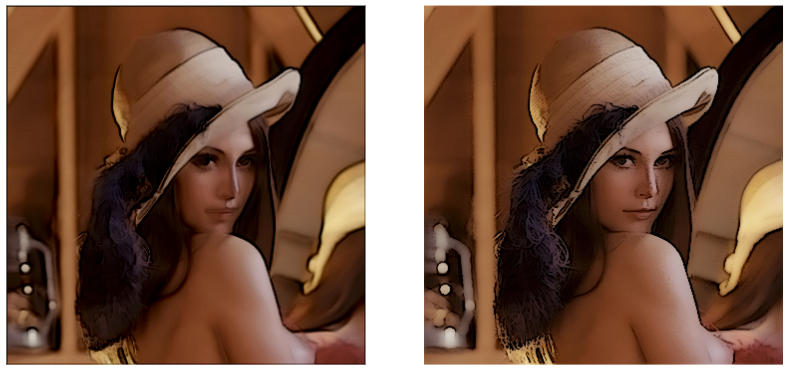
\includegraphics[width=1.0\textwidth]{edge-01.png}
\caption{Detektor hran - Sobel a LoG}
\end{figure}

Co se týče detekce hran, experimentoval jsem s LoG filtrem a aproximovanými jádry, které jsem zmiňoval v minulé sekci. V závislosti na velikosti matici se zvyšovala síla detekování a při větší matici jsem nedostával dobré výsledky. Nicméně jsem si vědom toho, že kdyby se mi podařilo správně naimplementovat LoG funkci a detekovat správně hrany (zero-crossings), tak bych dostával lepší výsledky.

\begin{figure}[!htb]
\centering
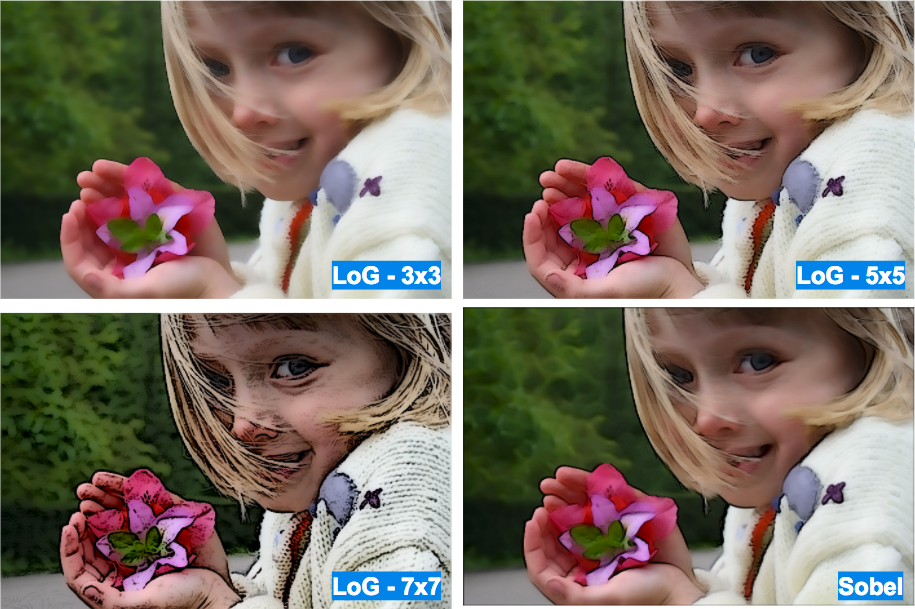
\includegraphics[width=1.0\textwidth]{edge-02.png}
\caption{Detektor hran - různá aproximovaná jádra u LoG a Sobel}
\end{figure}

\clearpage

\section{Závěr}
\par{V semestrální práci se mi podařilo naimplementovat bilaterální filtr, funkční detektor hran Sobel, dále funkci, která mi vrací matici podle Laplaciánu Gaussiánu, u které se mi však nepodařilo zprovoznit ji k detekování hran. Nakonec jsem použil aproximovaná jádra, se kterými se detekce hran zdařila. Poslední částí mé práce bylo funkční webové rozhraní pro vyfocení a upload obrázku, na který se následně dá použít několik filtrů.}

\par{Pokud bych měl v semestrální práci pokračovat, viděl bych hned několik věcí, které by se daly zlepšit - vylepšit LoG funkci a zařídit, aby fungovala u detekování hran, dále zrychlit výpočet bilaterálního filtru, který je v současnosti velmi pomalý (ideálně v reálném čase na GPU, aby bylo možné filtrovat živý záznam z webové kamery).}

\section*{Použité zdroje}
[1] SÝKORA, Daniel. Digital Image Processing: Linear Filtering (přednáška). Praha, ČVUT 2017.
\\ \
\\ \
[2] SÝKORA, Daniel. Digital Image Processing: Non-Linear Filtering (přednáška). Praha, ČVUT 2017.
\\ \
\\ \
[3] FISHER, Robert, PERKINS Simon, WALKER, Ashley a WOLFART, Erik. Laplacian/Laplacian of Gaussian \textit{[online]}. [cit. 2017-20-05]. Dostupné z: \textbf{http://homepages.inf.ed.ac.uk/rbf/HIPR2/log.htm}
\\ \
\\ \
[4] Hamamatsu Corporation. Image Processing and Analysis \textit{[online]}. [cit. 2017-20-05]. Dostupné z: \textbf{https://hcimage.com/help/Content/Quantitation/Measurements/\newline Processing\%20and\%20Analysis/Enhance/Enhance\%20Operations.htm}

\end{document}